%! TeX program = lualatex
\documentclass[a4paper]{article} 

% packages
\usepackage{microtype}      % Slightly tweak font spacing for aesthetics
\usepackage[english]{babel} % Language hyphenation and typographical rules
\usepackage[final, colorlinks = true, urlcolor = black, linkcolor = black]{hyperref} 
\usepackage{changepage}     % adjust margins on the fly

\usepackage{fontspec}
\setmainfont{EB Garamond}
\setmonofont[Scale=MatchLowercase]{Deja Vu Sans Mono}

\usepackage{minted}
\usemintedstyle{algol_nu}
\usepackage{xcolor}

\usepackage{pgfplots}
\pgfplotsset{width=\textwidth,compat=1.9}

\usepackage{caption}
\newenvironment{code}{\captionsetup{type=listing}}{}
\captionsetup[listing]{skip=0pt}
\setlength{\abovecaptionskip}{5pt}
\setlength{\belowcaptionskip}{5pt}

\usepackage[yyyymmdd]{datetime}
\renewcommand{\dateseparator}{--}

\usepackage{titlesec}
% \titleformat{\section}{\LARGE\bfseries}{}{}{}[\titlerule]
% \titleformat{\subsection}{\Large\bfseries}{}{0em}{}
% \titlespacing{\subsection}{0em}{-0.7em}{0em}
%
% \titleformat{\subsubsection}{\large\bfseries}{}{0em}{$\bullet$ }
% \titlespacing{\subsubsection}{1em}{-0.7em}{0em}

% margins
\addtolength{\hoffset}{-2.25cm}
\addtolength{\textwidth}{4.5cm}
\addtolength{\voffset}{-3.25cm}
\addtolength{\textheight}{5cm}
\setlength{\parskip}{0pt}
\setlength{\parindent}{0in}
% \setcounter{secnumdepth}{0}

\begin{document}
\hrule \medskip
\begin{minipage}{0.295\textwidth} 
    \raggedright
    \footnotesize 
    \begin{tabular}{@{}l l} % Define a two-column table with left alignment
        Name: & Andrew Hayes \\
        Student ID: & 21321503 \\
    \end{tabular}
\end{minipage}
\begin{minipage}{0.4\textwidth} 
    \centering 
    \vspace{0.4em}
    \LARGE 
    \textsc{ct404} \\ 
\end{minipage}
\begin{minipage}{0.295\textwidth} 
    \raggedleft
    \footnotesize 
    \begin{tabular}{@{}l l} % Define a two-column table with left alignment
        Name: & Brian Moyles \\
        Student ID: & 21333461\\
    \end{tabular}
\end{minipage}
\smallskip
\hrule 
\begin{center}
    \normalsize
    Lab Assignment 2: HOG
\end{center}
\hrule

\section{HOG Feature Extraction on Your Own Image (\mintinline{matlab}{cell_size=4}, \mintinline{matlab}{block_size=2})}
\noindent
\begin{minipage}{0.49\textwidth}
\begin{figure}[H]
    \centering
    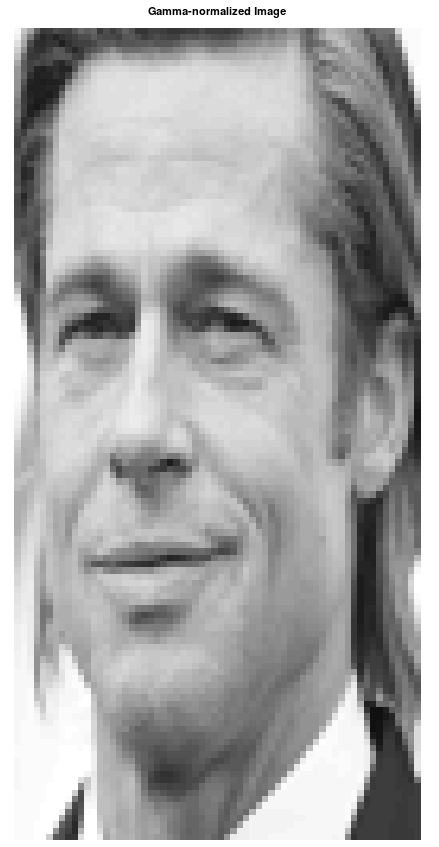
\includegraphics[width=0.6\textwidth]{./images/1_gamma-normalised.png}
    \caption{Gamma-normalised image}
\end{figure}
\end{minipage}
\hfill
\begin{minipage}{0.49\textwidth}
\begin{figure}[H]
    \centering
    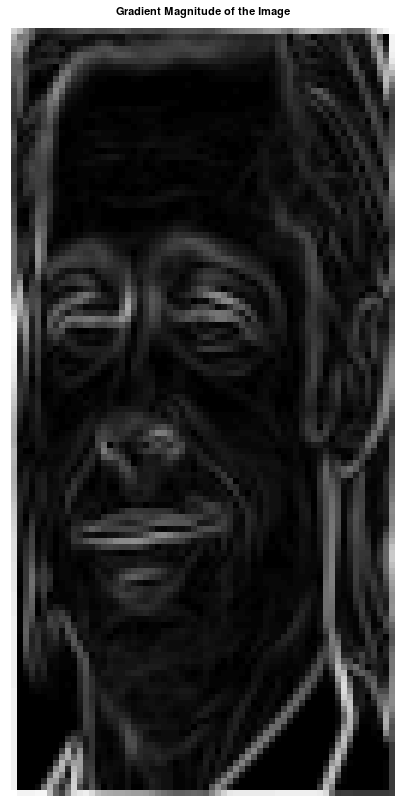
\includegraphics[width=0.6\textwidth]{./images/1_gradient_magnitude.png}
    \caption{Gradient magnitude of the image}
\end{figure}
\end{minipage}

\begin{minipage}{0.49\textwidth}
\begin{figure}[H]
    \centering
    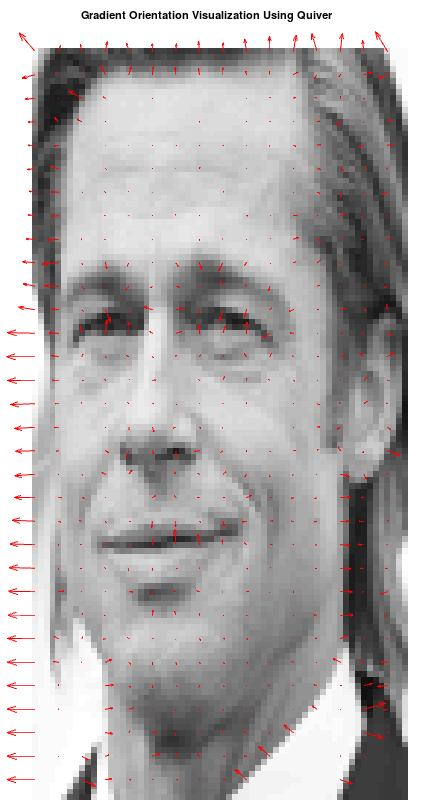
\includegraphics[width=0.6\textwidth]{./images/1_gradient_orientation.png}
    \caption{Gradient orientation visualisation using Quiver}
\end{figure}
\end{minipage}
\hfill
\begin{minipage}{0.49\textwidth}
\begin{figure}[H]
    \centering
    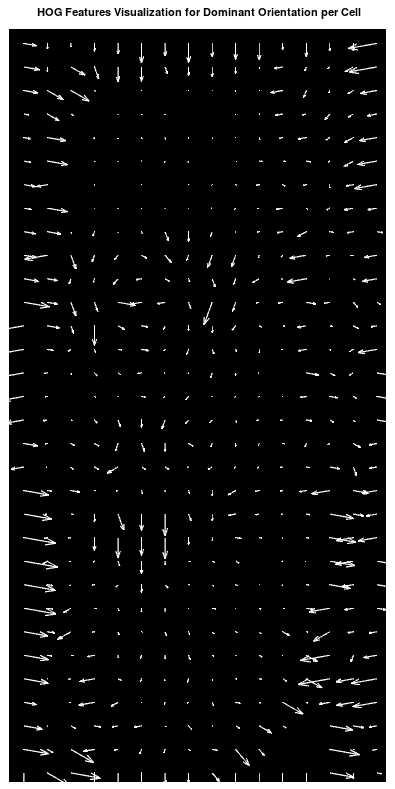
\includegraphics[width=0.6\textwidth]{./images/1_hog_features.png}
    \caption{HOG features visualisation for the dominant orientation per cell}
\end{figure}
\end{minipage}

\section{Experiment with HOG Parameters}
\subsection{\mintinline{matlab}{cell_size = 8}, \mintinline{matlab}{block_size=2}}
\noindent
\begin{minipage}{0.49\textwidth}
\begin{figure}[H]
    \centering
    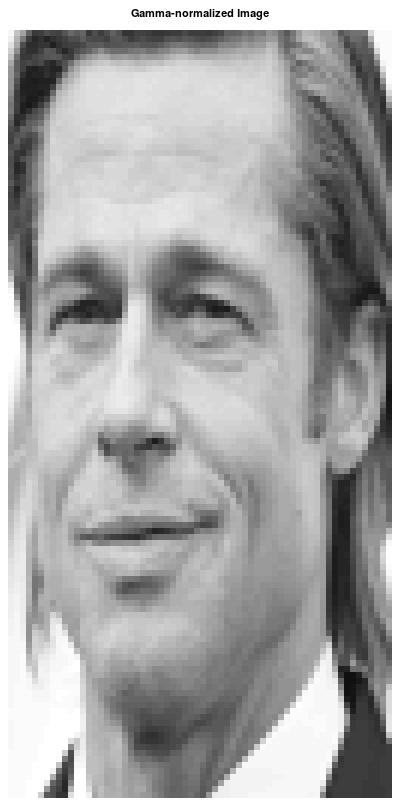
\includegraphics[width=0.6\textwidth]{./images/2_1_gamma-normalised.png}
    \caption{Gamma-normalised image}
\end{figure}
\end{minipage}
\hfill
\begin{minipage}{0.49\textwidth}
\begin{figure}[H]
    \centering
    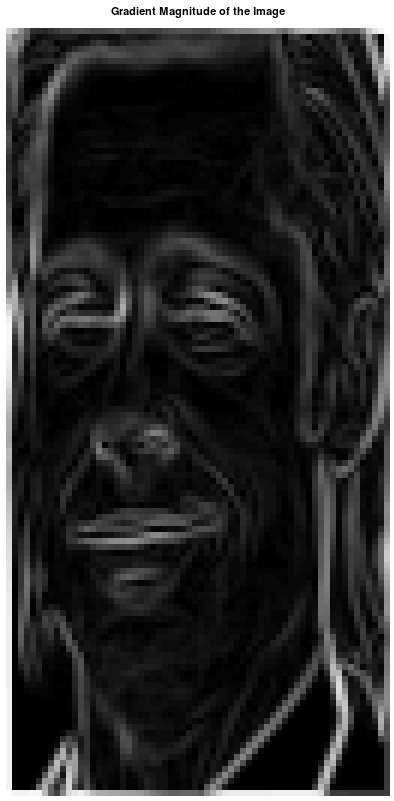
\includegraphics[width=0.6\textwidth]{./images/2_1_gradient_magnitude.png}
    \caption{Gradient magnitude of the image}
\end{figure}
\end{minipage}

\begin{minipage}{0.49\textwidth}
\begin{figure}[H]
    \centering
    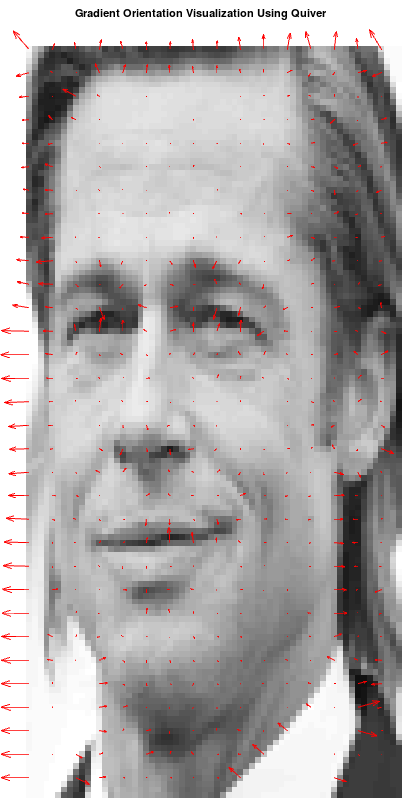
\includegraphics[width=0.6\textwidth]{./images/2_1_gradient_orientation.png}
    \caption{Gradient orientation visualisation using Quiver}
\end{figure}
\end{minipage}
\hfill
\begin{minipage}{0.49\textwidth}
\begin{figure}[H]
    \centering
    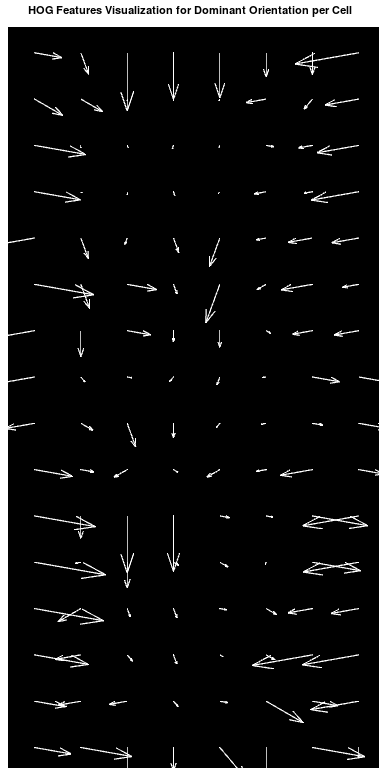
\includegraphics[width=0.6\textwidth]{./images/2_1_hog_features.png}
    \caption{HOG features visualisation for the dominant orientation per cell}
\end{figure}
\end{minipage}

\subsection{\mintinline{matlab}{cell_size = 16}, \mintinline{matlab}{block_size=4}}
\noindent
\begin{minipage}{0.49\textwidth}
\begin{figure}[H]
    \centering
    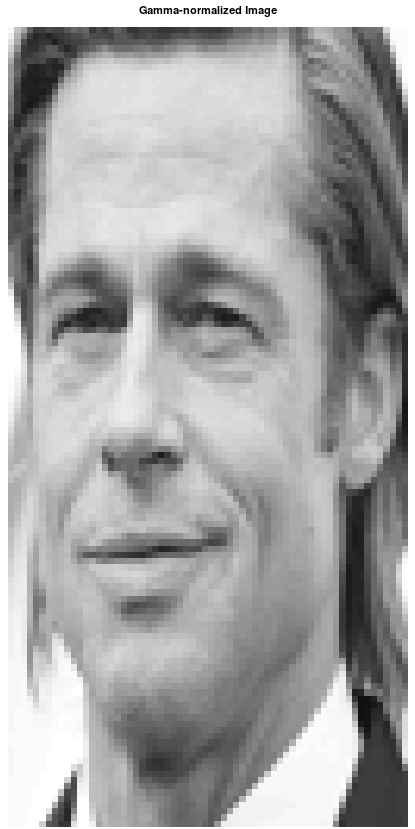
\includegraphics[width=0.6\textwidth]{./images/2_2_gamma-normalised.png}
    \caption{Gamma-normalised image}
\end{figure}
\end{minipage}
\hfill
\begin{minipage}{0.49\textwidth}
\begin{figure}[H]
    \centering
    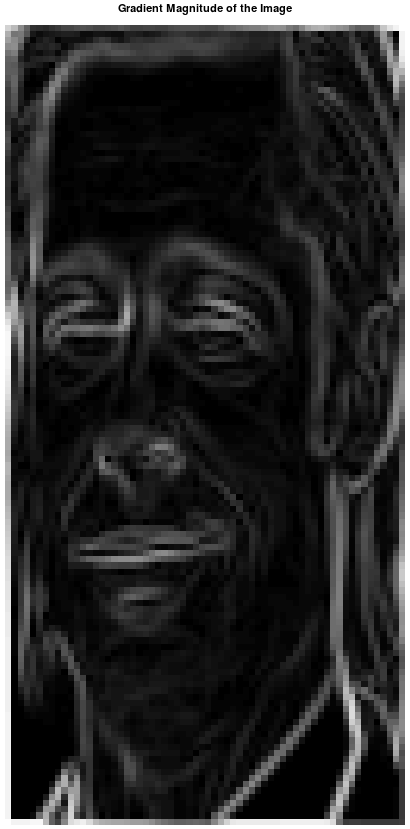
\includegraphics[width=0.6\textwidth]{./images/2_2_gradient_magnitude.png}
    \caption{Gradient magnitude of the image}
\end{figure}
\end{minipage}

\begin{minipage}{0.49\textwidth}
\begin{figure}[H]
    \centering
    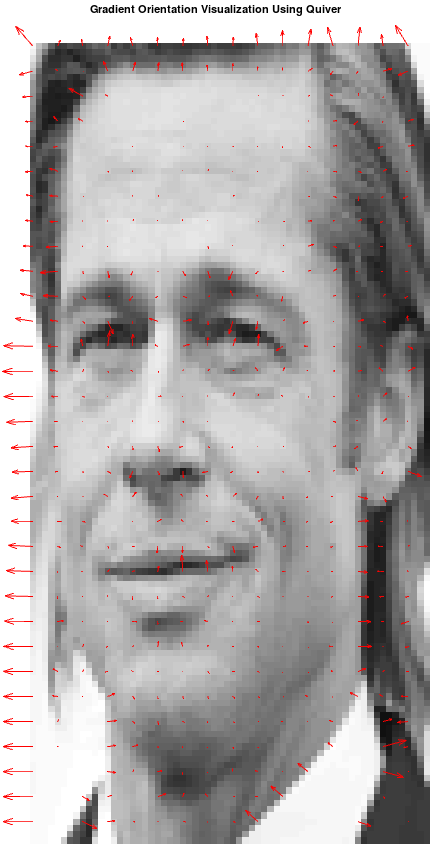
\includegraphics[width=0.6\textwidth]{./images/2_2_gradient_orientation.png}
    \caption{Gradient orientation visualisation using Quiver}
\end{figure}
\end{minipage}
\hfill
\begin{minipage}{0.49\textwidth}
\begin{figure}[H]
    \centering
    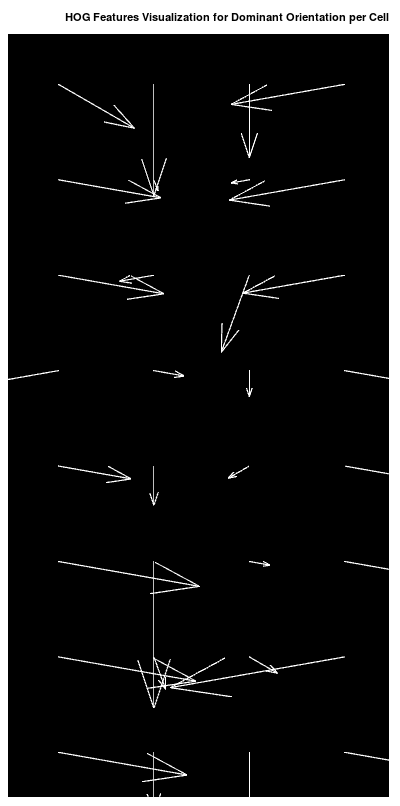
\includegraphics[width=0.6\textwidth]{./images/2_2_hog_features.png}
    \caption{HOG features visualisation for the dominant orientation per cell}
\end{figure}
\end{minipage}

\subsection{How does changing the cell size \& block size affect the HOG visualisation?}
A smaller cell size captures finer details \& small-scale gradients in the image, resulting in more local features and a dense \& detailed visualisation.
However, it's also more sensitive to noise, especially around the hair area where there are less prominent edges.
A larger cell size, on the other hand, results in a coarser representation with reduced sensitivity to small details \& noise, but with potential to miss finer-detailed structures like ears, and an overall sparser \& less detailed visualisation.
\\\\
A smaller block size focuses on local normalisation of gradient features, maintaining fine details and ensuring that local contrast variations are accounted for which can improve robustness in areas with significant intensity variation, such as around the eyes.
A larger block size averages features over a broader area, resulting in more ``global'' normalisation that can make it less sensitive to fine details \& noise.

\subsection{Which cell size \& block size provide the most visually distinguishable features?}
We would recommend the 8$\times$8 cell size with 2$\times$2 block size as it captures the important details \& overall structure of the face without introducing too much noise into the visualisation, without losing too much detail.
The original results obtained with \mintinline{matlab}{cell_size = 4}, \mintinline{matlab}{block_size=2} had a lot of noise compared to results obtained with \mintinline{matlab}{cell_size = 8}, \mintinline{matlab}{block_size=2}.
Furthermore, the results obtained with \mintinline{matlab}{cell_size = 16}, \mintinline{matlab}{block_size=4} were far too coarse to be visually distinguishable, and left out a lot of important details.

\section{HOG Feature Extraction on a Car or Truck Image}
\begin{figure}[H]
    \centering
    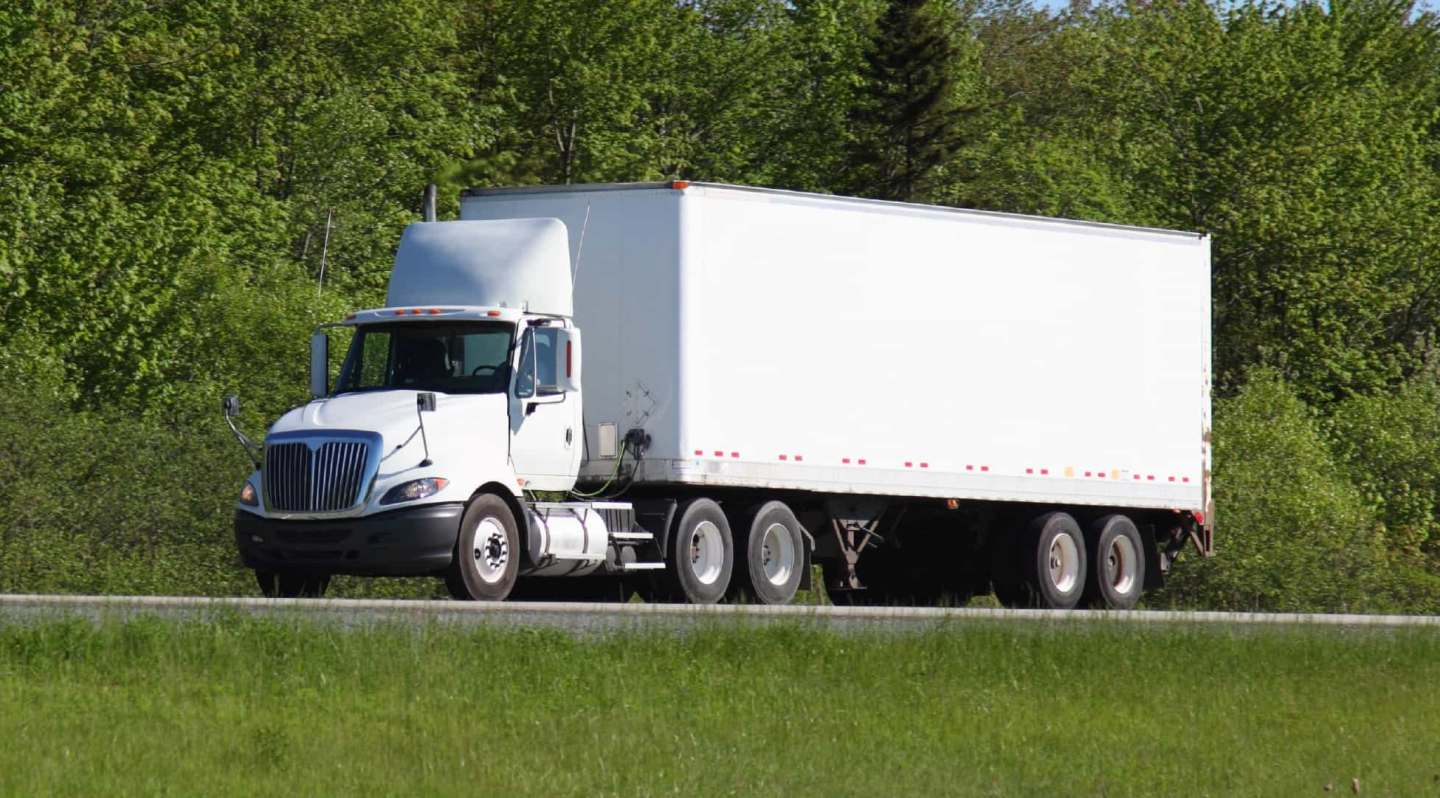
\includegraphics[width=0.6\textwidth]{../code/truck.jpg}
    \caption{Original truck image}
\end{figure}

\noindent
\begin{minipage}{0.49\textwidth}
\begin{figure}[H]
    \centering
    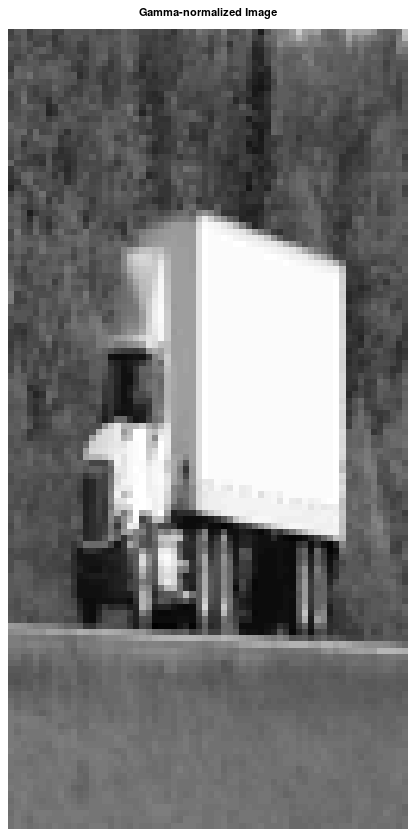
\includegraphics[width=0.6\textwidth]{./images/3_gamma-normalised.png}
    \caption{Gamma-normalised image}
\end{figure}
\end{minipage}
\hfill
\begin{minipage}{0.49\textwidth}
\begin{figure}[H]
    \centering
    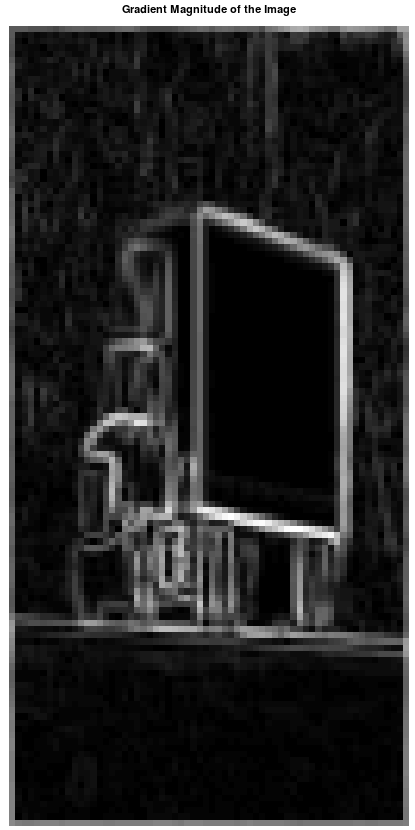
\includegraphics[width=0.6\textwidth]{./images/3_gradient_magnitude.png}
    \caption{Gradient magnitude of the image}
\end{figure}
\end{minipage}

\begin{minipage}{0.49\textwidth}
\begin{figure}[H]
    \centering
    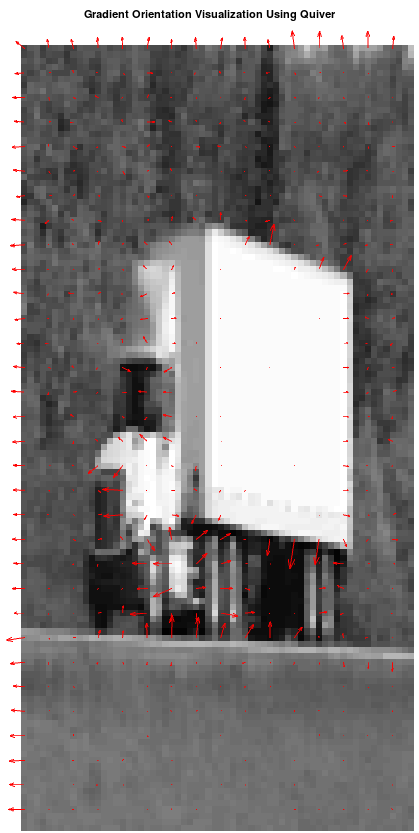
\includegraphics[width=0.6\textwidth]{./images/3_gradient_orientation.png}
    \caption{Gradient orientation visualisation using Quiver}
\end{figure}
\end{minipage}
\hfill
\begin{minipage}{0.49\textwidth}
\begin{figure}[H]
    \centering
    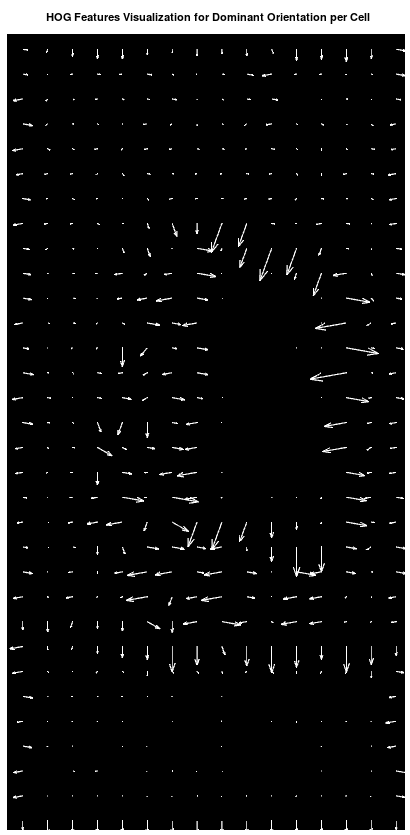
\includegraphics[width=0.6\textwidth]{./images/3_hog_features.png}
    \caption{HOG features visualisation for the dominant orientation per cell}
\end{figure}
\end{minipage}

\subsection{Differences in HOG Representation for Truck Image vs Face Image}
\begin{minipage}{0.49\textwidth}
\begin{figure}[H]
    \centering
    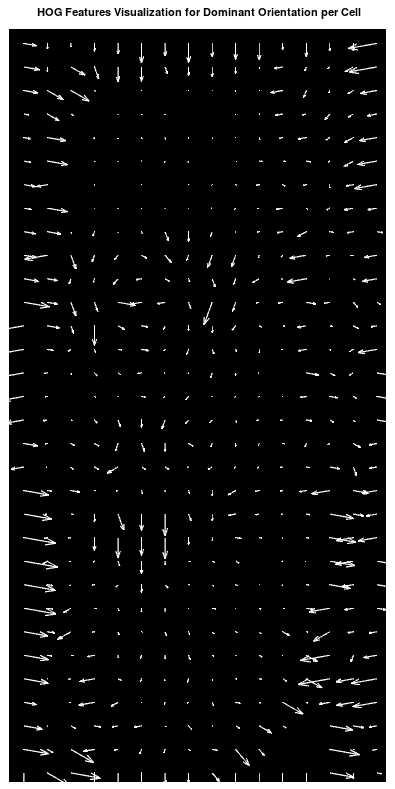
\includegraphics[width=0.6\textwidth]{./images/1_hog_features.png}
    \caption{HOG features visualisation for the face image}
\end{figure}
\end{minipage}
\hfill
\begin{minipage}{0.49\textwidth}
\begin{figure}[H]
    \centering
    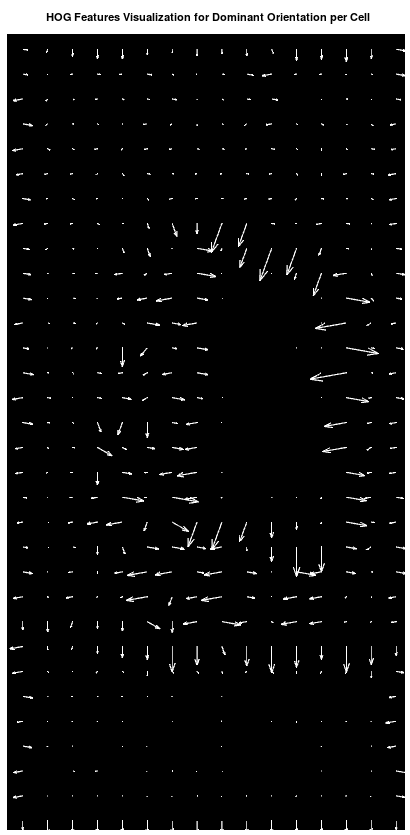
\includegraphics[width=0.6\textwidth]{./images/3_hog_features.png}
    \caption{HOG features visualisation for the truck image}
\end{figure}
\end{minipage}

The truck image contains a more straight lines than the face image, as it is an inorganic, regular object while the face image has more curved lines due to organic facial structure.
A large blank area can be seen in the HOG visualisation for the truck as the blank white side panel of the truck contains no edges or changes in intensity.
There is significantly less noise in the HOG visualisation for the truck due to the comparatively simpler \& more regular shape \& colours of the truck image.

\section{Conclusion}
\subsection{What effect did changing the \mintinline{matlab}{cell_size} \& \mintinline{matlab}{block_size} parameters have on the HOG features?}
Increasing the cell sizes \& block sizes reduced noise in the resulting HOG visualisations, but began to also remove important details \& features of the image as the cell size \& block size were further increased.

\subsection{How did the HOG features of your face compare to those of a car/truck?}
The HOG features of the face were significantly noisier, had greater curvature, and were less regular than the HOG features of the truck image due to one being a natural object and the other being man-made.

\subsection{Which parameter settings do you think would work best for distinguishing between different types of images?}
We would recommend the 8$\times$8 cell size with 2$\times$2 block size as it captures the important details \& overall structure of the face without introducing too much noise into the visualisation, without losing too much detail.

\end{document}
